Dans un premier temps, pour démoduler le signal, nous allons le filtrer. En effet, nous savons que les bits 0 sont modulés à une fréquence $F_0 = 6000Hz$, et les bits 1 sont modulés à une fréquence $F_1 = 2000Hz$.
Ainsi, en implémentant un filtre passe-bas pour commencer, nous filtrerons tous les bits 0, il ne restera plus que les bits 1, et nous saurons alors reconstruire le signal. Nous allons faire pareil avec un filtre passe-haut, qui ne gardera que les bits 0.

Pour cela nous définissons d'abord une fréquence de coupure \textcolor{Red}{\lstinline{Fc = 4500} $Hz$}, l'\textcolor{Red}{\lstinline{ordre = 101}} du filtre, et le
\textcolor{Red}{\lstinline{retard}}
\begin{lstlisting}
Fc = 4500;
Ordre = 101;
Retard = (Ordre - 1) / 2;   
\end{lstlisting}
\subsubsection{Filtre passe-bas}
Nous choisissons un simple sinus cardinal comme filtre.

\begin{lstlisting}[caption=Filtre passe-bas]
h_bas = 2 * Fc * Te * sinc(2 * Fc * Te * (-Retard:Retard));
H_bas = fft(h_bas);
y_bas_retarde = filter(h_bas, 1, [x zeros(1, Retard)]);
y_bas = y_bas_retarde(Retard + 1:end);
\end{lstlisting}

La ligne 4 permet de ne pas perdre de données. La ligne 5 permet de supprimer le retard.
Voici les résultats que nous avons obtenus :
\begin{dinglist}{111}
   \item \textbf{Réponses du filtre.}
   Voici les réponses fréquentielle et impultionnelle du filtre passe-bas.
   Notez que les lignes en pointillés sur la Figure \ref{fig : rep-bas}.\ref{sub@fig:rep-freq-bas} marquent la fréquence de coupure $F_c = 4500 Hz$.
   \begin{figure}[H]
      \centering
      \begin{subfigure}{0.5\textwidth}
         \centering
         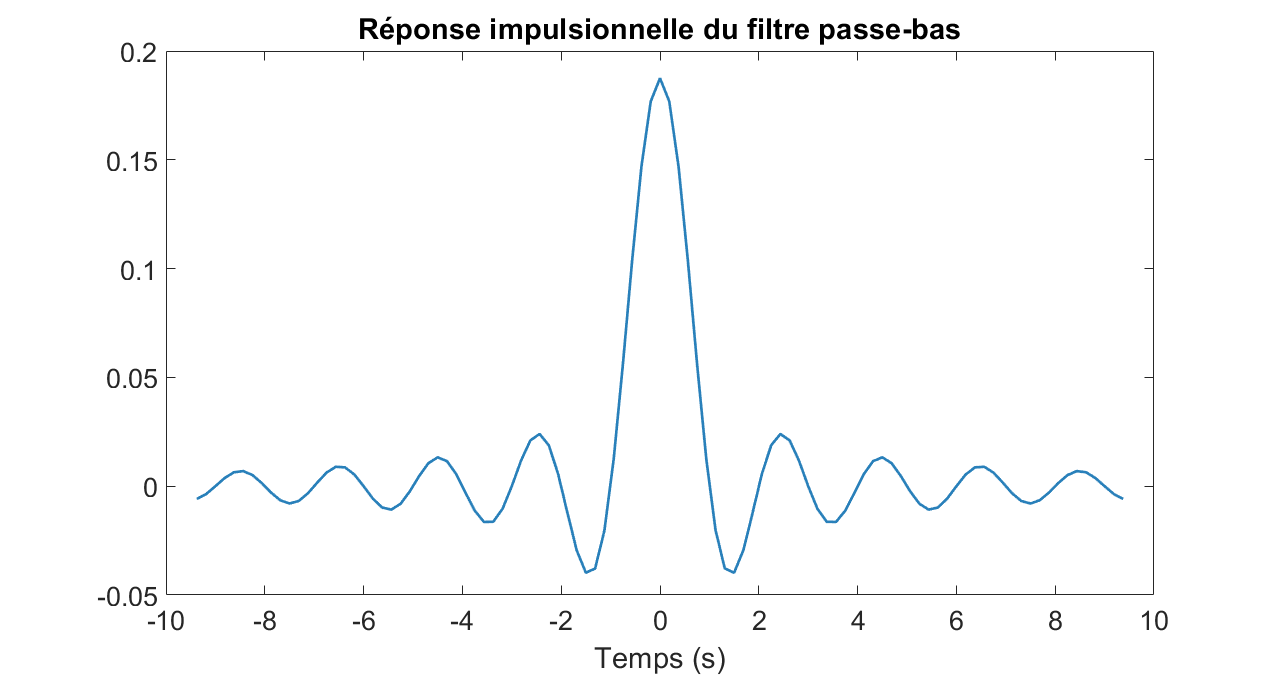
\includegraphics[width=\textwidth]{partie-2/sous-partie-3/2.3.3.1.png}
         \caption{Réponse impultionnelle du filtre passe-bas} \label{fig:rep-imp-bas}
      \end{subfigure}%
      \begin{subfigure}{0.5\textwidth}
         \centering
         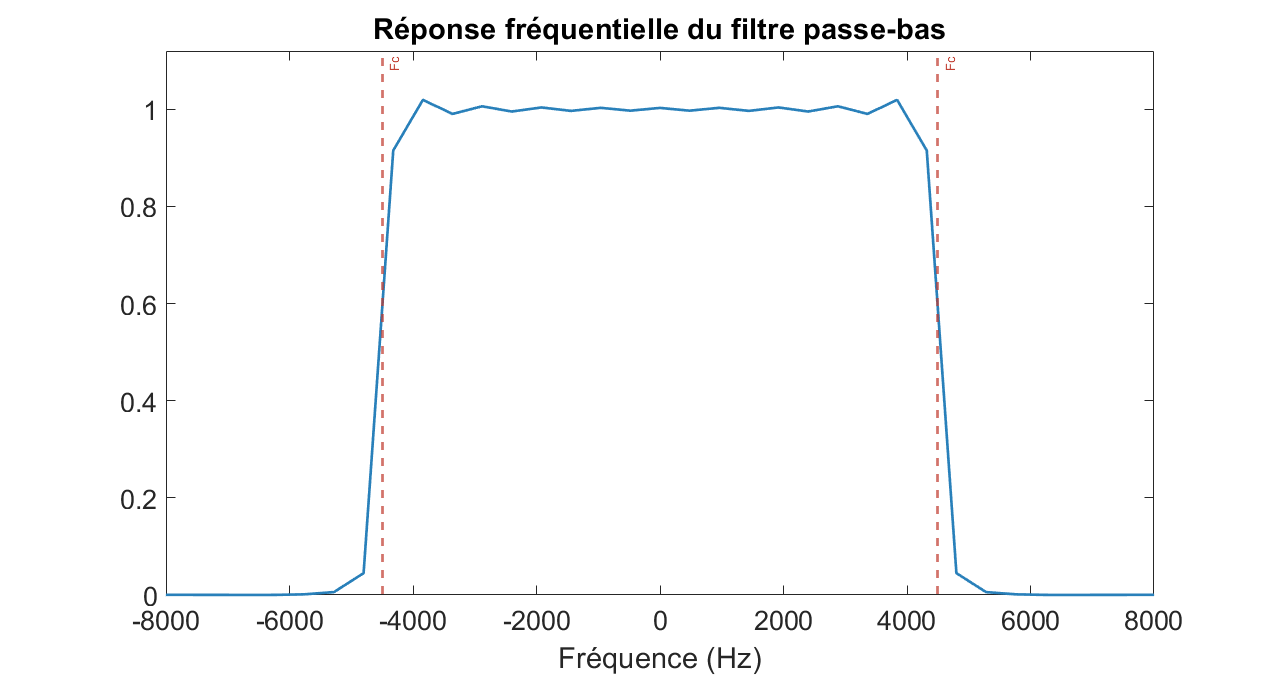
\includegraphics[width=\textwidth]{partie-2/sous-partie-3/2.3.3.2.png}
         \caption{Réponse fréquentielle du filtre passe-bas}\label{fig:rep-freq-bas}
      \end{subfigure}
      \caption{Réponses du filtre passe-bas \label{fig : rep-bas}}
   \end{figure}
   \item \textbf{Densité spectrale de puissance du signal non filtré.}
   \begin{figure}[H]
      \centering
      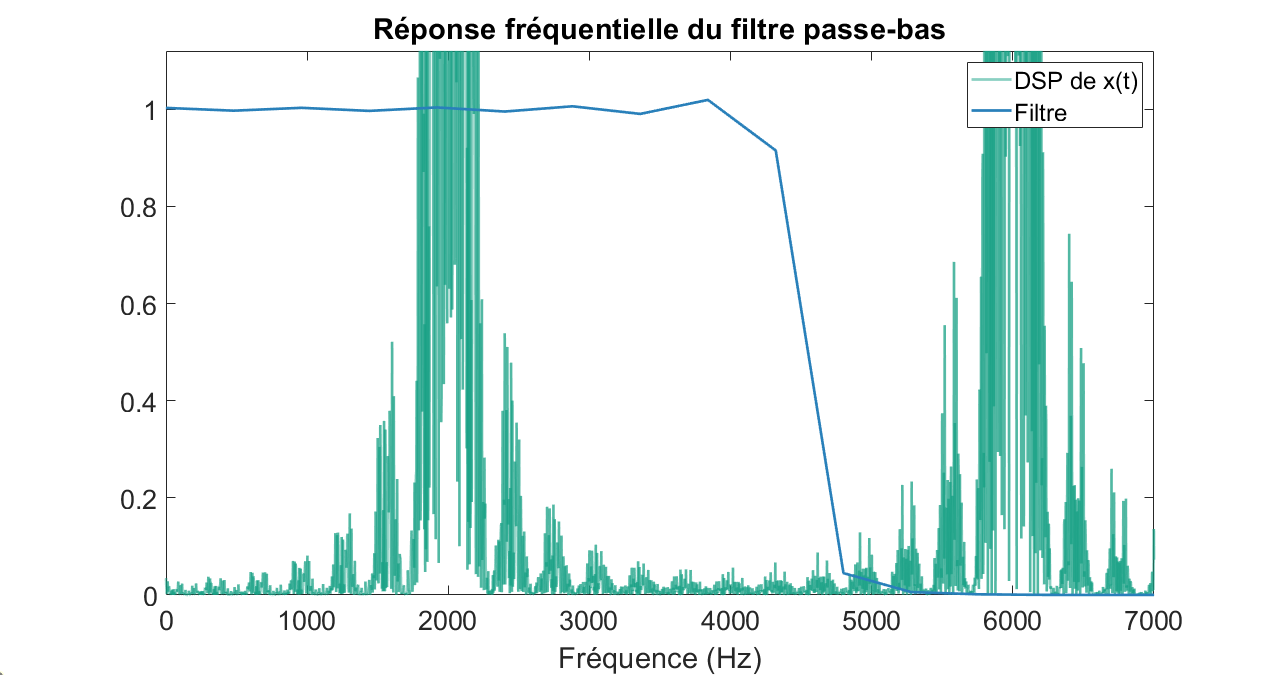
\includegraphics[width=\textwidth]{partie-2/sous-partie-3/2.3.3.3.png}
      \caption{Densité spectrale de puissance du signal non filtré (passe-bas)} \label{fig:spb-nn-filtre-bas}
   \end{figure}
   Nous pouvons voir que le filtre coupe bien les hautes fréquences, notamment les fréquences autour de 6000 Hz, représentant les bits 0. La démodulation va donc bien petre possible.

   \item \textbf{Signal filtré.}
   \begin{figure}[H]
      \centering
      \begin{subfigure}{0.5\textwidth}
         \centering
         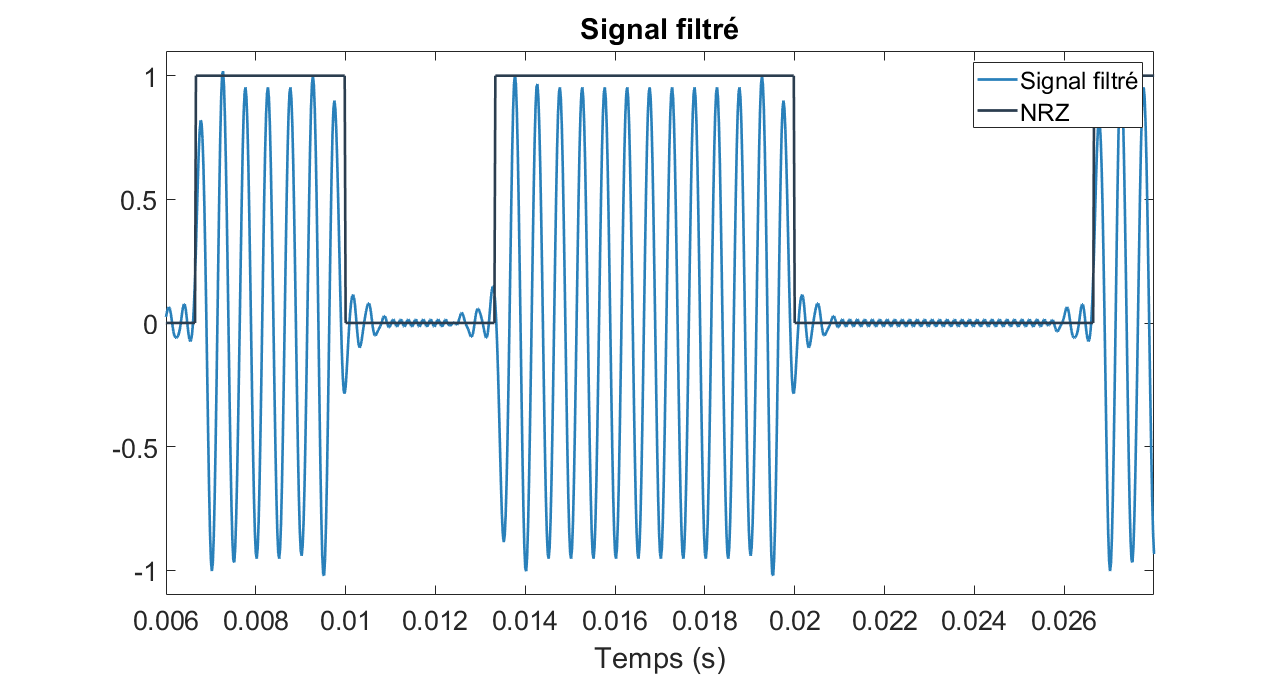
\includegraphics[width=\textwidth]{partie-2/sous-partie-3/2.3.3.4.png}
         \caption{Signal filtré} \label{fig:filtre-temp-bas}
      \end{subfigure}%
      \begin{subfigure}{0.5\textwidth}
         \centering
         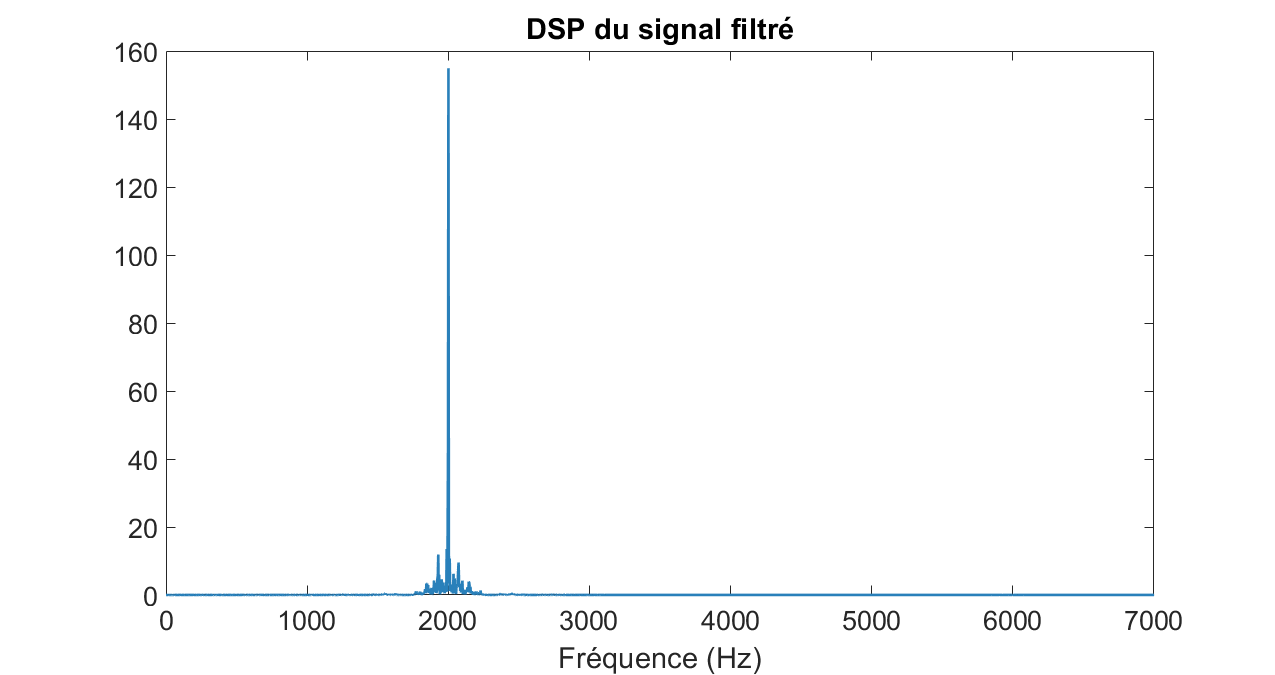
\includegraphics[width=\textwidth]{partie-2/sous-partie-3/2.3.3.5.png}
         \caption{DSP du signal filtré}\label{fig:filtre-freq-bas}
      \end{subfigure}
      \caption{Signal filtré (passe-bas)\label{fig:signal-filtre-bas}}
   \end{figure}
   Nous remarquons que le signal a été filtré comme voulu :
   \begin{itemize}
      \item les bits 0 sont filtrés (Figure \ref{fig:signal-filtre-bas}.\ref{sub@fig:filtre-temp-bas})
      \item les hautes fréquences ont été coupées, il ne reste plus que les fréquences inférieures à 4500Hz (Figure \ref{fig:signal-filtre-bas}.\ref{sub@fig:filtre-freq-bas})
   \end{itemize}
\end{dinglist}





\subsubsection{Filtre passe-haut}
De manière similaire, nous implémentons le filtre passe-haut.

\begin{lstlisting}[caption=Filtre passe-haut]
h_haut = -h_bas;
h_haut(Retard) = 1 - Fc / Fe;
H_haut = fft(h_haut);
y_haut_retarde = filter(h_haut, 1, [x zeros(1, Retard)]);
y_haut = y_haut_retarde(Retard + 1:end);
\end{lstlisting}
Et voici les résultats :

\begin{dinglist}{111}
   \item \textbf{Réponses du filtre.}
   Voici les réponses fréquentielle et impultionnelle du filtre passe-haut.
   De même,les lignes en pointillés sur la Figure \ref{fig : rep-haut}.\ref{sub@fig:rep-freq-haut} marquent la fréquence de coupure $F_c = 4500 Hz$.
   \begin{figure}[H]
      \centering
      \begin{subfigure}{0.5\textwidth}
         \centering
         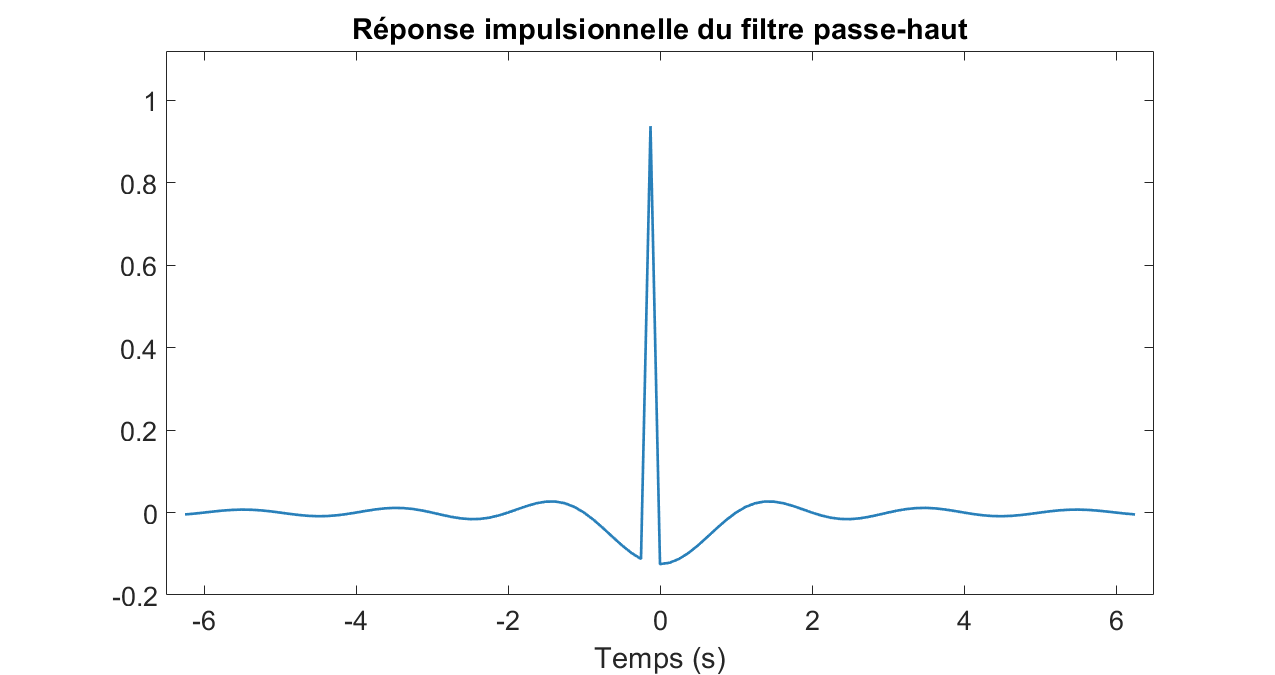
\includegraphics[width=\textwidth]{partie-2/sous-partie-3/2.3.3.6.png}
         \caption{Réponse impultionnelle du filtre passe-haut} \label{fig:rep-imp-haut}
      \end{subfigure}%
      \begin{subfigure}{0.5\textwidth}
         \centering
         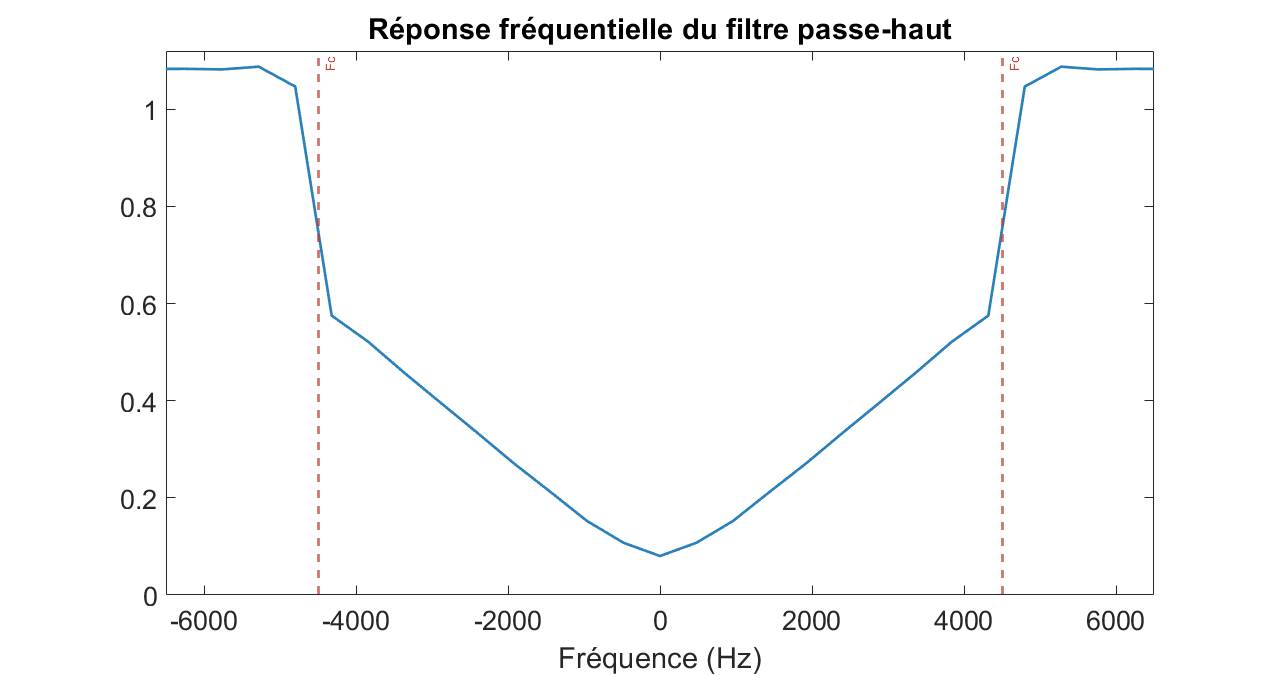
\includegraphics[width=\textwidth]{partie-2/sous-partie-3/2.3.3.7.png}
         \caption{Réponse fréquentielle du filtre passe-haut}\label{fig:rep-freq-haut}
      \end{subfigure}
      \caption{Réponses du filtre passe-haut \label{fig : rep-haut}}
   \end{figure}
   \item \textbf{Densité spectrale de puissance du signal non filtré.}
   \begin{figure}[H]
      \centering
      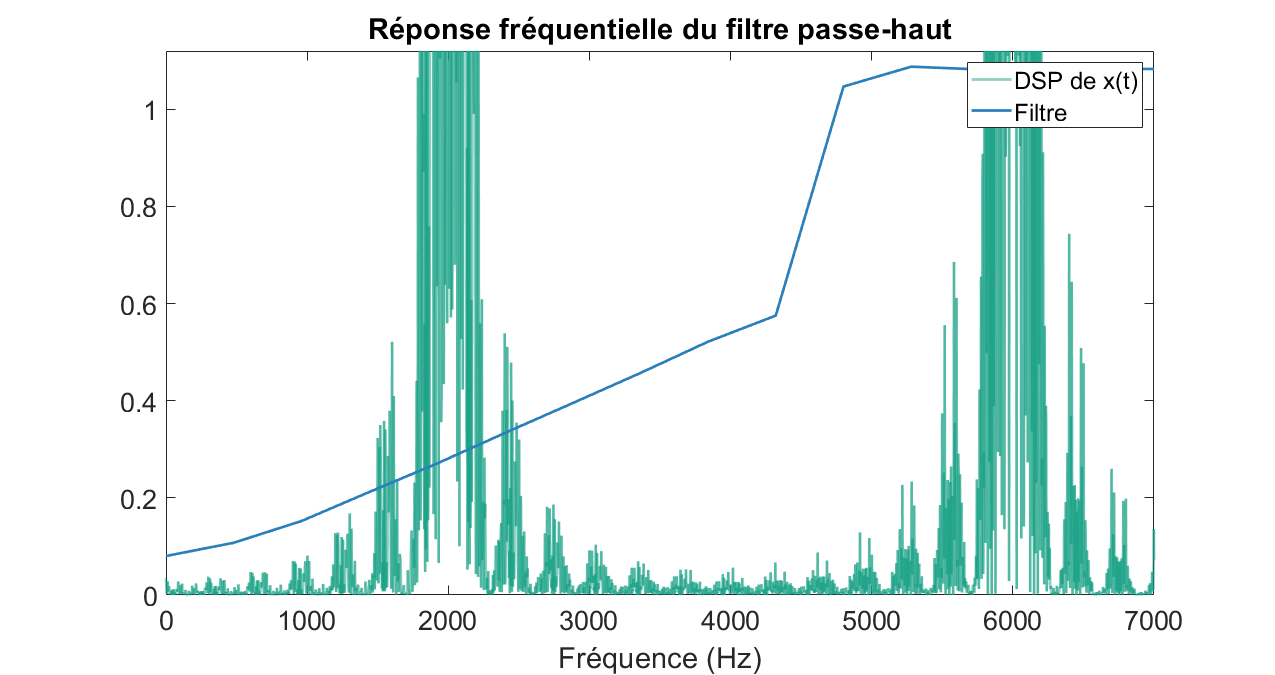
\includegraphics[width=\textwidth]{partie-2/sous-partie-3/2.3.3.8.png}
      \caption{Densité spectrale de puissance du signal non filtré (passe-haut)} \label{fig:spb-nn-filtre-haut}
   \end{figure}
   On remarque cette fois-ci que le filtre ne permet pas de couper toutes les fréquences basses, la démodulation sera toujours possible, mais moins bien.

   \item \textbf{Signal filtré.}
   \begin{figure}[H]
      \centering
      \begin{subfigure}{0.5\textwidth}
         \centering
         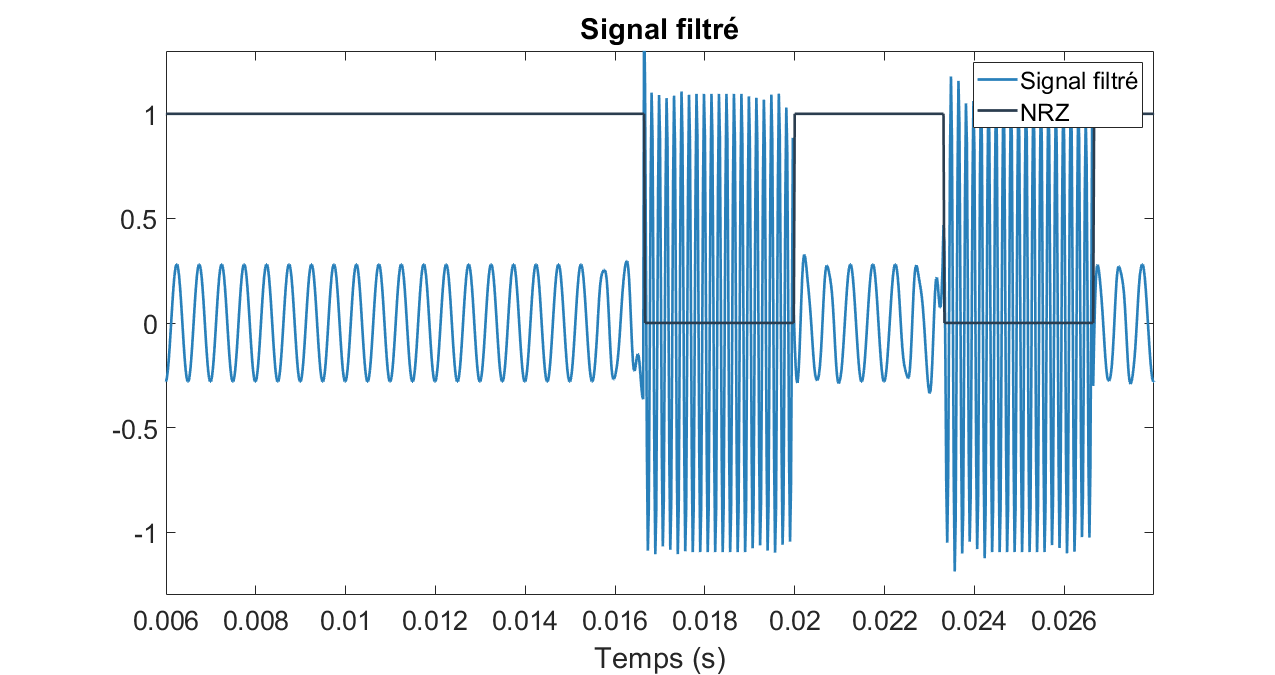
\includegraphics[width=\textwidth]{partie-2/sous-partie-3/2.3.3.9.png}
         \caption{Signal filtré} \label{fig:filtre-temp-haut}
      \end{subfigure}%
      \begin{subfigure}{0.5\textwidth}
         \centering
         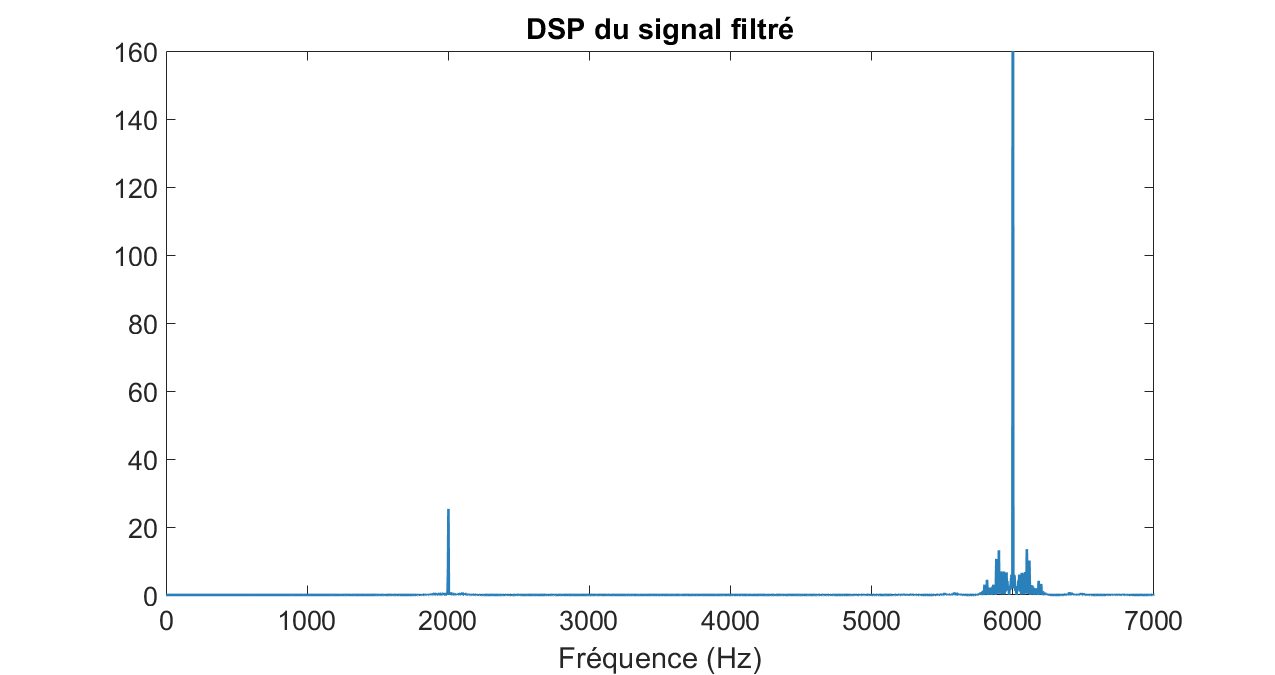
\includegraphics[width=\textwidth]{partie-2/sous-partie-3/2.3.3.10.png}
         \caption{DSP du signal filtré}\label{fig:filtre-freq-haut}
      \end{subfigure}
      \caption{Signal filtré (passe-haut) \label{fig:signal-filtre-haut}}
   \end{figure}
   On voit bien que tout n'est pas filtré, par exemple sur la Figure  \ref{fig:signal-filtre-haut}.\ref{sub@fig:filtre-temp-haut}, on voit qu'il reste des fréquences autour de 2000 Hz. Mais les bits 1 ont une amplitude beaucoup plus faible que les bits 0 (Figure \ref{fig:signal-filtre-haut}.\ref{sub@fig:filtre-temp-haut}). La démodulation sera donc correcte.
\end{dinglist}


\subsubsection{Détection d'énergie}
Il ne reste maintenant plus qu'à traduire le signal modulé en une suite de bits (0 et 1).
Nous décidons de garder notre signal filtré par le passe-bas.
Pour cela on utilise un détecteur d'énergie :
\begin{itemize}
   \item sur la durée d'un bit $T_s$, on mesure l'énergie du signal.
   \item si cette énergie est supérieure à un seuil $K$, alors le bit est 1
\end{itemize}
Note : l'énergie d'un signal $X = \left\{x_i ; i\in\llbracket1,N_s\rrbracket\right\}$ de $N_s$ échantillons se calcule selon :
\[
   \sum_{n=1}^{N_s} x_n^2
\]
\begin{lstlisting}[caption=Détection d'énergie]
K = 11; % seuil d'energie determine experimentalement
y_redecoupe = reshape(y_bas, Ns, Nb_bit);
X = sum(y_redecoupe.^2, 1);
Donnee_retrouve = X > K;
\end{lstlisting}
De plus, puisque nous connaissons le signal avant perturbation, nous pouvons calculer le taux d'erreur, en comparant le signal initial, et le signal reconstruit :
\begin{lstlisting}[caption=Taux d'erreur]
Nb_erreur = sum(Donnee ~= Donnee_retrouve);
taux_erreur = Nb_erreur / Nb_bit;
\end{lstlisting}

Nous obtenons ainsi un \textbf{\textcolor{Red}{taux d'erreur nul}}.

\subsubsection{Reconstitution de l'image codée}
Nous pouvons maintenant décoder l'image codée pour deviner le lieu et le personnage :
\begin{lstlisting}[caption=Reconstitution de l'image]
load DonneesBinome1.mat;
Nb_bit = 84000;
Donnee = bits;
...
reconstitution_image(Donnee_retrouve);
\end{lstlisting}
\begin{figure}[H]
   \centering
   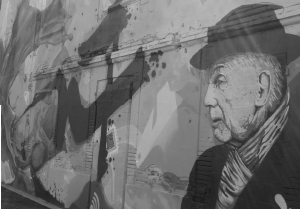
\includegraphics[scale=0.4]{partie-2/sous-partie-3/2.3.3.11.png}
   \caption{Image reconstituée} \label{fig:image-reconstituee}
\end{figure}

Nous reconnaissons ainsi le graphe représentant \textbf{\textcolor{Red}{Charles Camichel}} dans \textbf{\textcolor{Red}{la cours de l'école}}.

\subsubsection{Application à la recommandation V21}
Si nous voulons respecter la recommandation V21, nous devons maintenant changer les fréquences associées aux bits 0 et 1 :
\begin{dinglist}{111}
   \item $F_0$ = 1 180 Hz
   \item $F_1$ = 980 Hz
\end{dinglist}

Nous nous doutons que les filtres implantés ne pourront plus distinguer les bits, car leur fréquences seront trop rapprochées.
En effet, en changeant la fréquence de coupures, nous obtenons une taux d'erreur faible, mais non nul.
\begin{figure}[H]
   \centering
   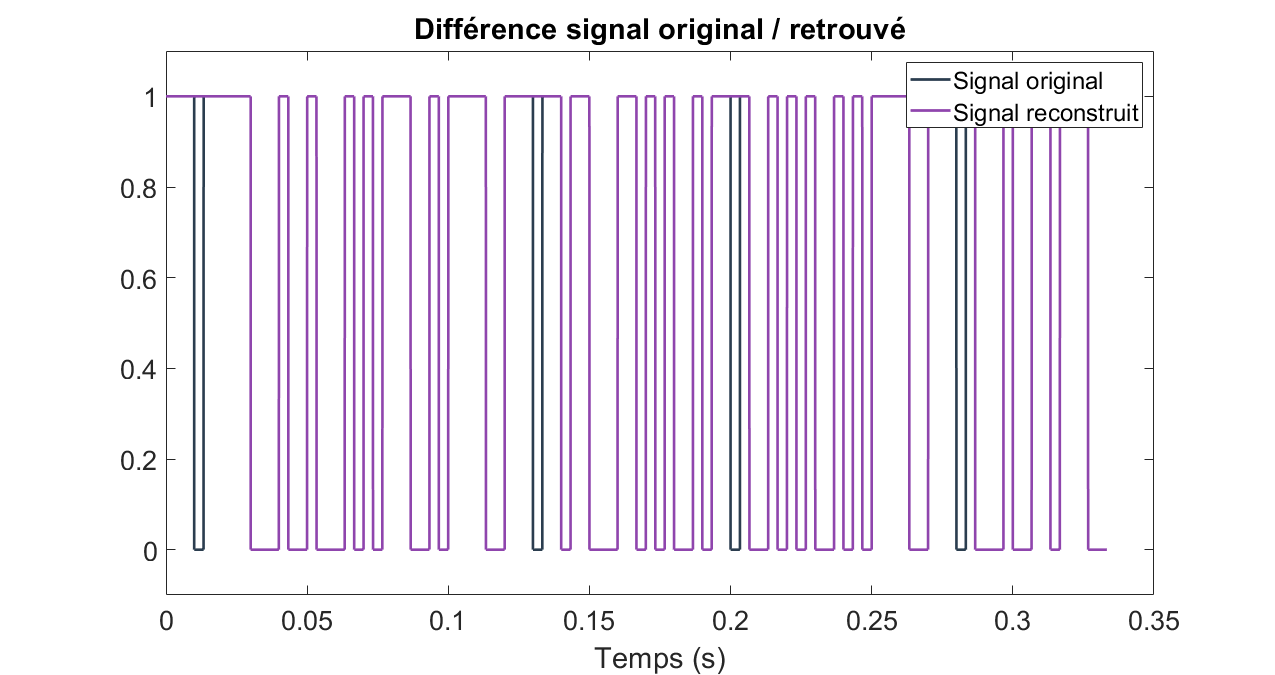
\includegraphics[scale=0.4]{partie-2/sous-partie-3/2.3.3.12.png}
   \caption{Signal reconstitué pour un taux d'erreur de 4\%} \label{fig:image-reconstituee}
\end{figure}